\section{August 24, 2026}

\subsection{Ordinary differential equations}

An ODE has the form
\[
  x'(t)=f(t,x(t)).
\]
Given an initial condition $x(t_0)=x_0$, the corresponding
\emph{initial-value problem} (IVP) is to find $x(t)$ for $t\geq t_0$ such
that
\begin{equation}\label{eq:ivp}
  x'(t)=f(t,x(t)),
  \qquad
  x(t_0)=x_0.
\end{equation}

Topics arising in the numerical solution of differential equations include
\begin{itemize}
  \item non-stiff problems and stiff solvers;
  \item geometric solvers;
  \item parameter estimation and Bayesian approaches, where the vector
    field may depend on a model parameter $\theta$, as in $f(t,x,\theta)$;
  \item boundary-value problems; and
  \item stochastic differential equations (SDEs).
\end{itemize}

We generally consider vector-valued solutions and vector fields,
\[
  x\colon \bb{R}\longrightarrow \bb{R}^n,
  \qquad
  f\colon \bb{R}\times\bb{R}^n\longrightarrow\bb{R}^n,
\]
which can be written componentwise as
\[
  x=
  \begin{bmatrix}
    x_1\\ \vdots\\ x_n
  \end{bmatrix},
  \qquad
  f(t,x)=
  \begin{bmatrix}
    f_1(t,x_1,\ldots,x_n)\\
    \vdots\\
    f_n(t,x_1,\ldots,x_n)
  \end{bmatrix}.
\]

\subsection{Examples}

\begin{example}
  The scalar equation
  \[
    x'=x
  \]
  is an ODE with $n=1$.
\end{example}

\begin{example}[Damped oscillator]
  Consider the second-order equation
  \[
    x''=-\omega^2x-x'.
  \]
  Setting $x_1=x$ and $x_2=x'$ converts it into the first-order system
  \[
    \begin{cases}
      x_1'=x_2,\\
      x_2'=-\omega^2x_1-x_2.
    \end{cases}
  \]
  Thus, with $\mathbf{x}=(x_1,x_2)^{\mathsf T}$, we have
  $\mathbf{x}'=\mathbf{f}(x_1,x_2)$.
\end{example}

\begin{example}[Chemical kinetics]
  A three-species kinetic model is
  \[
    \mathbf{x}=
    \begin{bmatrix}
      x_1\\x_2\\x_3
    \end{bmatrix},
    \qquad
    \begin{cases}
      x_1'=-k_1x_1+k_2x_2x_3,\\
      x_2'= k_1x_1-k_2x_2x_3-k_3x_2^2,\\
      x_3'= k_3x_2^2,
    \end{cases}
  \]
  where $k_1,k_2,k_3>0$ are reaction rates. The reaction rates may occur
  on very different scales, which can lead to stiffness.
\end{example}

\begin{example}[Molecular model]
  Let $q_i$ be the position of particle $i$, let $m_i$ be its mass, and
  let $V(q_1,\ldots,q_N)$ be the potential energy. Newton's equation is
  \[
    m_iq_i''=-\frac{\partial V(q_1,\ldots,q_N)}{\partial q_i}.
  \]
  Introducing the momentum $p_i=m_iq_i'$ gives
  \[
    \begin{cases}
      q_i'=\dfrac{p_i}{m_i},\\[6pt]
      p_i'=-\dfrac{\partial V}{\partial q_i}.
    \end{cases}
  \]
  The positions and momenta can therefore be collected into the state
  vector
  \[
    \mathbf{x}=
    \begin{bmatrix}
      q_1\\p_1\\q_2\\p_2\\\vdots\\q_N\\p_N
    \end{bmatrix}.
  \]

  \begin{center}
    \begin{tikzpicture}[scale=0.85]
      \foreach \point in {(-2,0),(-1.2,0.9),(-0.8,-0.8),(0.2,0.45),
                           (1.1,-0.45),(1.8,0.65)}
        \fill \point circle (1.6pt);
      \fill (-2,0) circle (2.5pt) node[below left] {$i$};
      \draw[->,thick] (-2,0) -- (-0.35,1.25) node[above] {$q_i$};
    \end{tikzpicture}
  \end{center}
\end{example}

\subsection{Solutions and the Lipschitz condition}

Consider the IVP \eqref{eq:ivp} on an interval containing $t_0$.

\begin{definition}
  A function $x(t)$ is a \emph{solution} of the IVP if it satisfies the
  integral equation
  \[
    x(t)=x_0+\int_{t_0}^t f(s,x(s))\,ds.
  \]
\end{definition}

\begin{definition}[Lipschitz condition]
  The vector field $f$ is \emph{Lipschitz continuous in $x$} on a domain
  $D$ if there is a constant $L\geq 0$ such that
  \[
    \lVert f(t,x)-f(t,y)\rVert
    \leq L\lVert x-y\rVert
  \]
  for all $x,y\in D$ and all relevant $t$.
\end{definition}

Under the usual continuity assumption in $t$, the Lipschitz condition in
$x$ implies that the solution of the IVP exists and is unique on an
appropriate interval.

The same condition also controls the sensitivity to the initial data. Let
$x(t)$ and $y(t)$ be solutions with initial values $x_0$ and $y_0$,
respectively. Their integral equations give
\begin{align*}
  \lVert x(t)-y(t)\rVert
  &\leq \lVert x_0-y_0\rVert
    +\int_{t_0}^t
      \lVert f(s,x(s))-f(s,y(s))\rVert\,ds\\
  &\leq \lVert x_0-y_0\rVert
    +L\int_{t_0}^t\lVert x(s)-y(s)\rVert\,ds.
\end{align*}
By Gr\"onwall's inequality,
\begin{equation}\label{eq:gronwall-stability}
  \lVert x(t)-y(t)\rVert
  \leq \lVert x_0-y_0\rVert e^{L(t-t_0)}.
\end{equation}

\begin{center}
  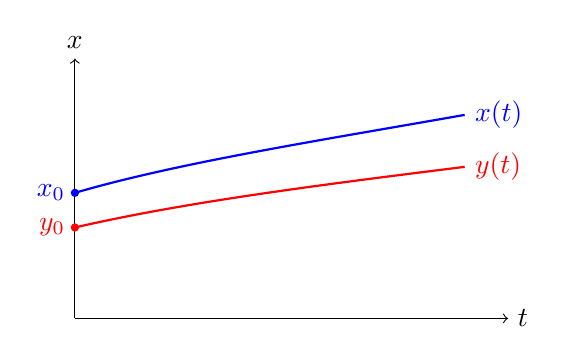
\begin{tikzpicture}[x=1.1cm,y=1.1cm]
    \draw[->] (0,0) -- (5,0) node[right] {$t$};
    \draw[->] (0,0) -- (0,3) node[above] {$x$};
    \draw[blue,thick] (0,1.45) .. controls (1.2,1.8) and (2.8,2.05) ..
      (4.5,2.35) node[right] {$x(t)$};
    \draw[red,thick] (0,1.05) .. controls (1.3,1.35) and (2.9,1.55) ..
      (4.5,1.75) node[right] {$y(t)$};
    \fill[blue] (0,1.45) circle (1.5pt) node[left] {$x_0$};
    \fill[red] (0,1.05) circle (1.5pt) node[left] {$y_0$};
  \end{tikzpicture}
\end{center}

Thus nearby initial values produce solutions whose separation is bounded
by \eqref{eq:gronwall-stability}.
